\chapter{Raw Data}
\section{ตัวอย่างไฟล์ CSV ที่ได้จาก UWB}
Tree 1: \\
\verb|pc_time,esp_time,tag_id,range_m,rx_power_dbm| \\
\texttt{2026-03-14T11:39:00,152,A49C,12.463,-96.76} \\
\texttt{2026-03-14T11:39:01,153,A49C,12.509,-95.31} \\
\texttt{2026-03-14T11:39:02,154,A49C,12.538,-95.86} \\
\texttt{2026-03-14T11:39:03,155,A49C,12.556,-99.77} \\
\texttt{2026-03-14T11:39:04,156,A49C,12.598,-101.1} \\
\\Tree 2: \\
\verb|pc_time,esp_time,tag_id,range_m,rx_power_dbm| \\
\texttt{2026-03-14T11:39:59,211,A49C,12.047,-90.55} \\
\texttt{2026-03-14T11:40:00,212,A49C,11.952,-89.25} \\
\texttt{2026-03-14T11:40:01,213,A49C,11.915,-88.94} \\
\texttt{2026-03-14T11:40:02,214,A49C,11.889,-92.35} \\
\texttt{2026-03-14T11:40:03,215,A49C,11.838,-82.43} \\
\\Tree 3: \\
\verb|pc_time,esp_time,tag_id,range_m,rx_power_dbm| \\
\texttt{2026-03-14T11:45:30,150,A49C,13.393,-96.59} \\
\texttt{2026-03-14T11:45:31,151,A49C,13.381,-97.28} \\
\texttt{2026-03-14T11:45:33,152,A49C,13.369,-96.78} \\
\texttt{2026-03-14T11:45:34,154,A49C,13.36,-97.56} \\
\texttt{2026-03-14T11:45:35,155,A49C,13.371,-98.48} \\

\chapter{Source Code}
บทนี้จะนำเสนอ Source Code ที่ใช้ในระบบ รวมถึงโปรแกรมวัดระยะ UWB สำหรับอุปกรณ์ Anchor และ Tag ตลอดจนสคริปต์บันทึกข้อมูลที่เขียนด้วยภาษา Python
\section{Anchor Program}
โปรแกรม \texttt{anchor.ino} ใช้สำหรับควบคุมโมดูล ESP32 UWB ที่ทำหน้าที่เป็น Anchor โดยทำการวัดระยะทางจาก Tag และคำนวณค่าเฉลี่ยภายในช่วงเวลา 1 วินาที เพื่อลดสัญญาณรบกวนของข้อมูล

\begin{lstlisting}[language=C]
#define DRONE_OFFSET 0.0148
#define WARMUP_TIME 5000

float sumRange = 0;
float sumRx = 0;
int sampleCount = 0;
unsigned long windowStart = 0;

void newRange()
{
  if (millis() - startTime < WARMUP_TIME)
    return;

  DW1000Device* dev = DW1000Ranging.getDistantDevice();

  float r  = dev->getRange();
  float rx = dev->getRXPower();

  if (r <= 0 || r > 100)
    return;

  float corrected = r - DRONE_OFFSET;

  if (windowStart == 0)
    windowStart = millis();

  sumRange += corrected;
  sumRx += rx;
  sampleCount++;

  if (millis() - windowStart >= 1000)
  {
    float avgRange = (sumRange / sampleCount) - 0.75;
    float avgRx = sumRx / sampleCount;

    Serial.print(windowStart / 1000);
    Serial.print(",");
    Serial.print(dev->getShortAddress(), HEX);
    Serial.print(",");
    Serial.print(avgRange, 3);
    Serial.print(",");
    Serial.println(avgRx, 2);

    sumRange = 0;
    sumRx = 0;
    sampleCount = 0;
    windowStart = millis();
  }
}
\end{lstlisting}

\section{Tag Program}
โปรแกรม \texttt{tag.ino} ใช้สำหรับกำหนดให้อุปกรณ์ ESP32 UWB ทำหน้าที่เป็น Tag โดยทำการส่งสัญญาณไปยัง Anchor เพื่อใช้ในการวัดระยะทาง

\begin{lstlisting}[language=C]
void dummyRange() {
  // Required callback for DW1000 state machine
}

void setup()
{
  Serial.begin(115200);

  SPI.begin(SPI_SCK, SPI_MISO, SPI_MOSI);
  DW1000Ranging.initCommunication(PIN_RST, PIN_SS, PIN_IRQ);

  DW1000Ranging.attachNewRange(dummyRange);
  DW1000Ranging.useRangeFilter(true);

  DW1000Ranging.startAsTag(
    TAG_ADD,
    DW1000.MODE_LONGDATA_RANGE_LOWPOWER
  );
}

void loop()
{
  DW1000Ranging.loop();
}
\end{lstlisting}

\section{Data Logging Script}
สคริปต์ \texttt{write\_file.py} ใช้สำหรับบันทึกข้อมูลที่ได้รับจาก Anchor ผ่าน Serial Port และจัดเก็บในรูปแบบไฟล์ CSV โดยมีการบันทึกเวลาจากเครื่องคอมพิวเตอร์ร่วมกับข้อมูลที่ได้รับจาก ESP32

\begin{lstlisting}[language=Python]
PORT = "COM3"   # Anchor Port
BAUD = 115200

ser = serial.Serial(PORT, BAUD, timeout=1)

writer.writerow([
    "pc_time",
    "esp_time",
    "tag_id",
    "range_m",
    "rx_power_dbm"
])

while True:
    line = ser.readline().decode(errors="ignore").strip()

    if not line:
        continue

    data = line.split(",")
    if len(data) != 4:
        continue

    pc_time = datetime.now().isoformat(timespec="seconds")

    writer.writerow([
        pc_time,
        data[0],
        data[1],
        data[2],
        data[3],
    ])
\end{lstlisting}

\chapter{Additional Figures}
ภาคผนวกนี้นำเสนอภาพประกอบเพิ่มเติมที่เกี่ยวข้องกับกระบวนการทดลองและการประมวลผลข้อมูล เพื่อสนับสนุนความเข้าใจในขั้นตอนการดำเนินงานและการวิเคราะห์ผลลัพธ์
\section{ภาพการกำหนดพื้นที่ถ่ายภาพทางอากาศ}
\begin{figure}[H]
    \centering
    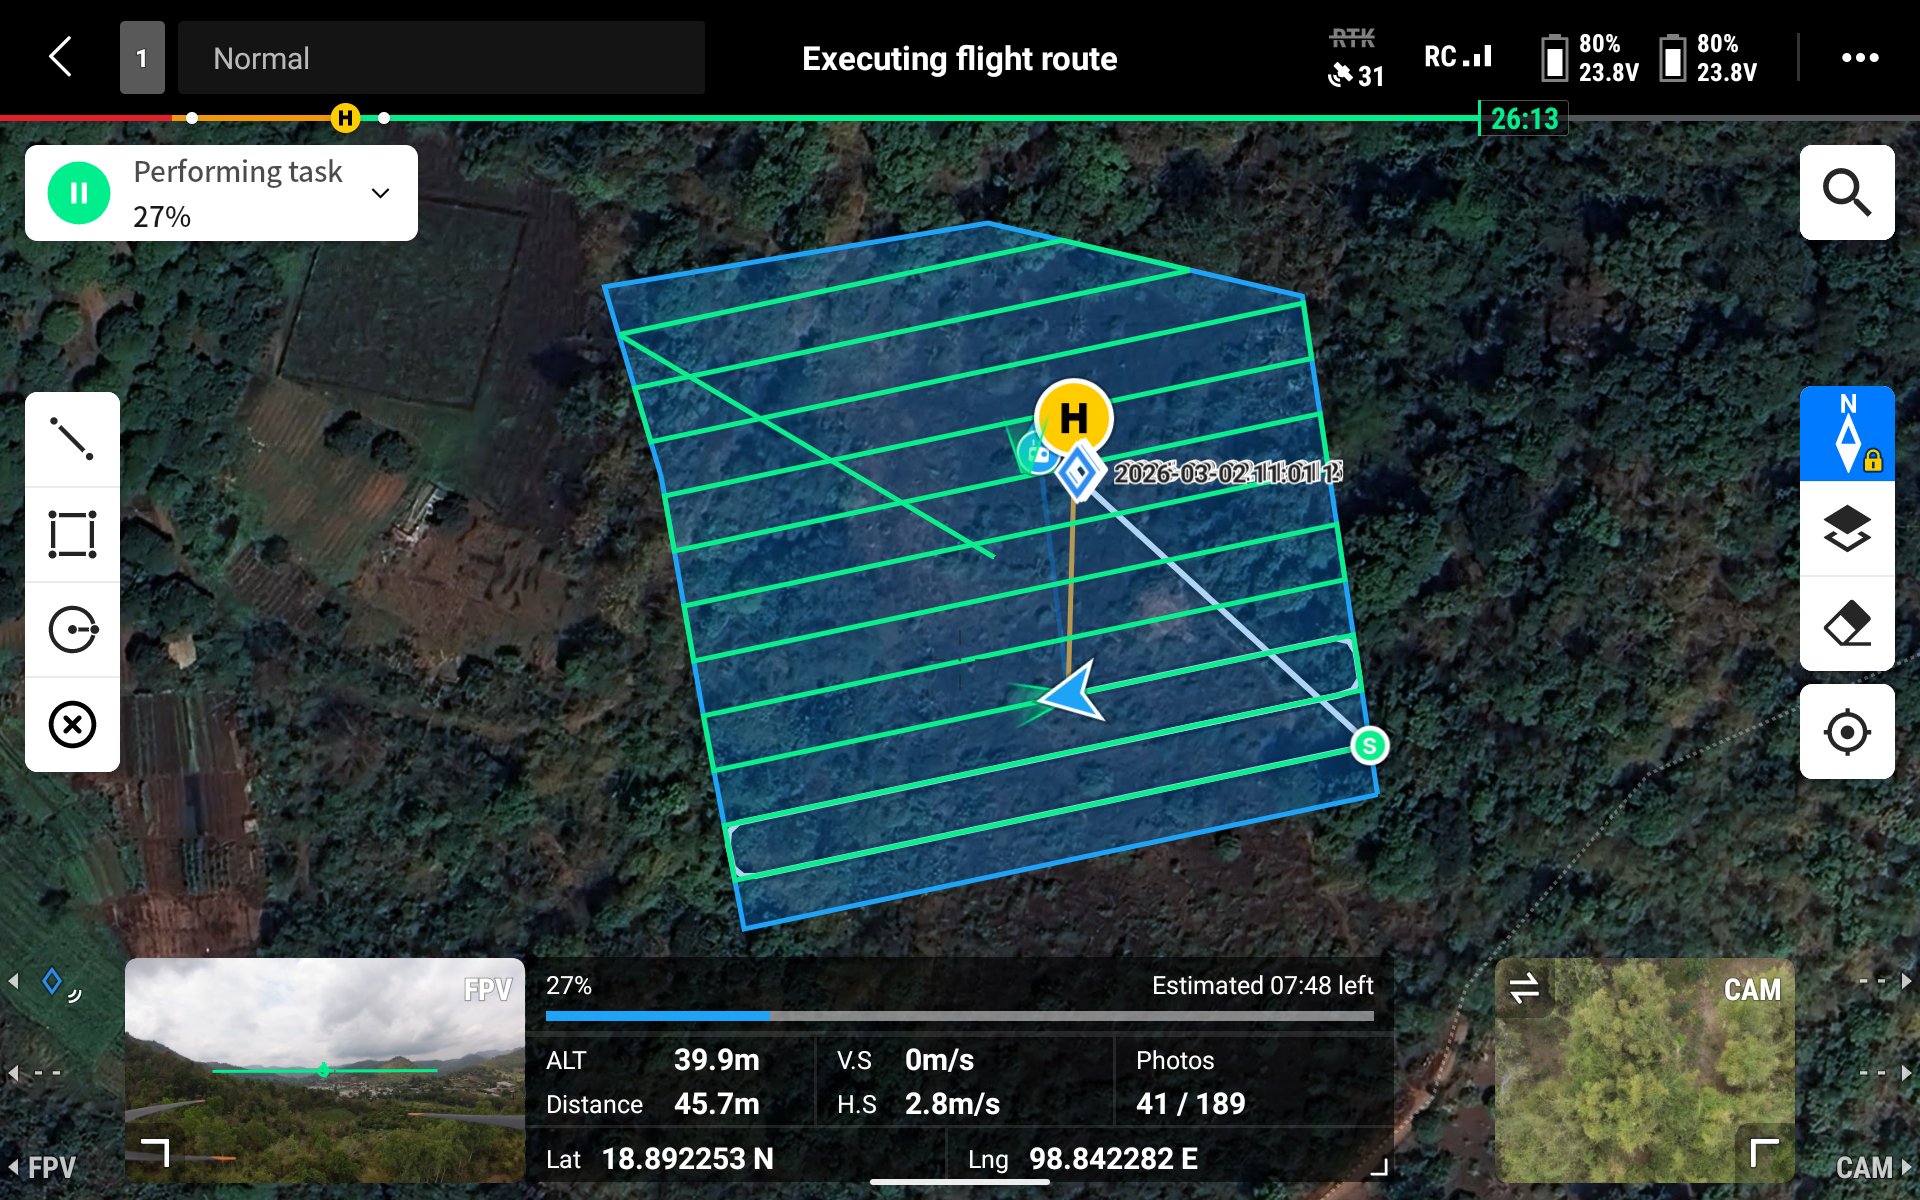
\includegraphics[width=0.6\linewidth]{fig/area.png}
    \caption{ภาพหน้าจอรีโมทของโดรนขณะกำหนดพื้นที่สำหรับการถ่ายภาพทางอากาศ เพื่อใช้ในการสร้างแบบจำลอง 3D Point Cloud}
    \label{fig:area}
\end{figure}

\section{ภาพการวัดระยะจาก VPS เหนือยอดไม้}
\begin{figure}[H]
    \centering
    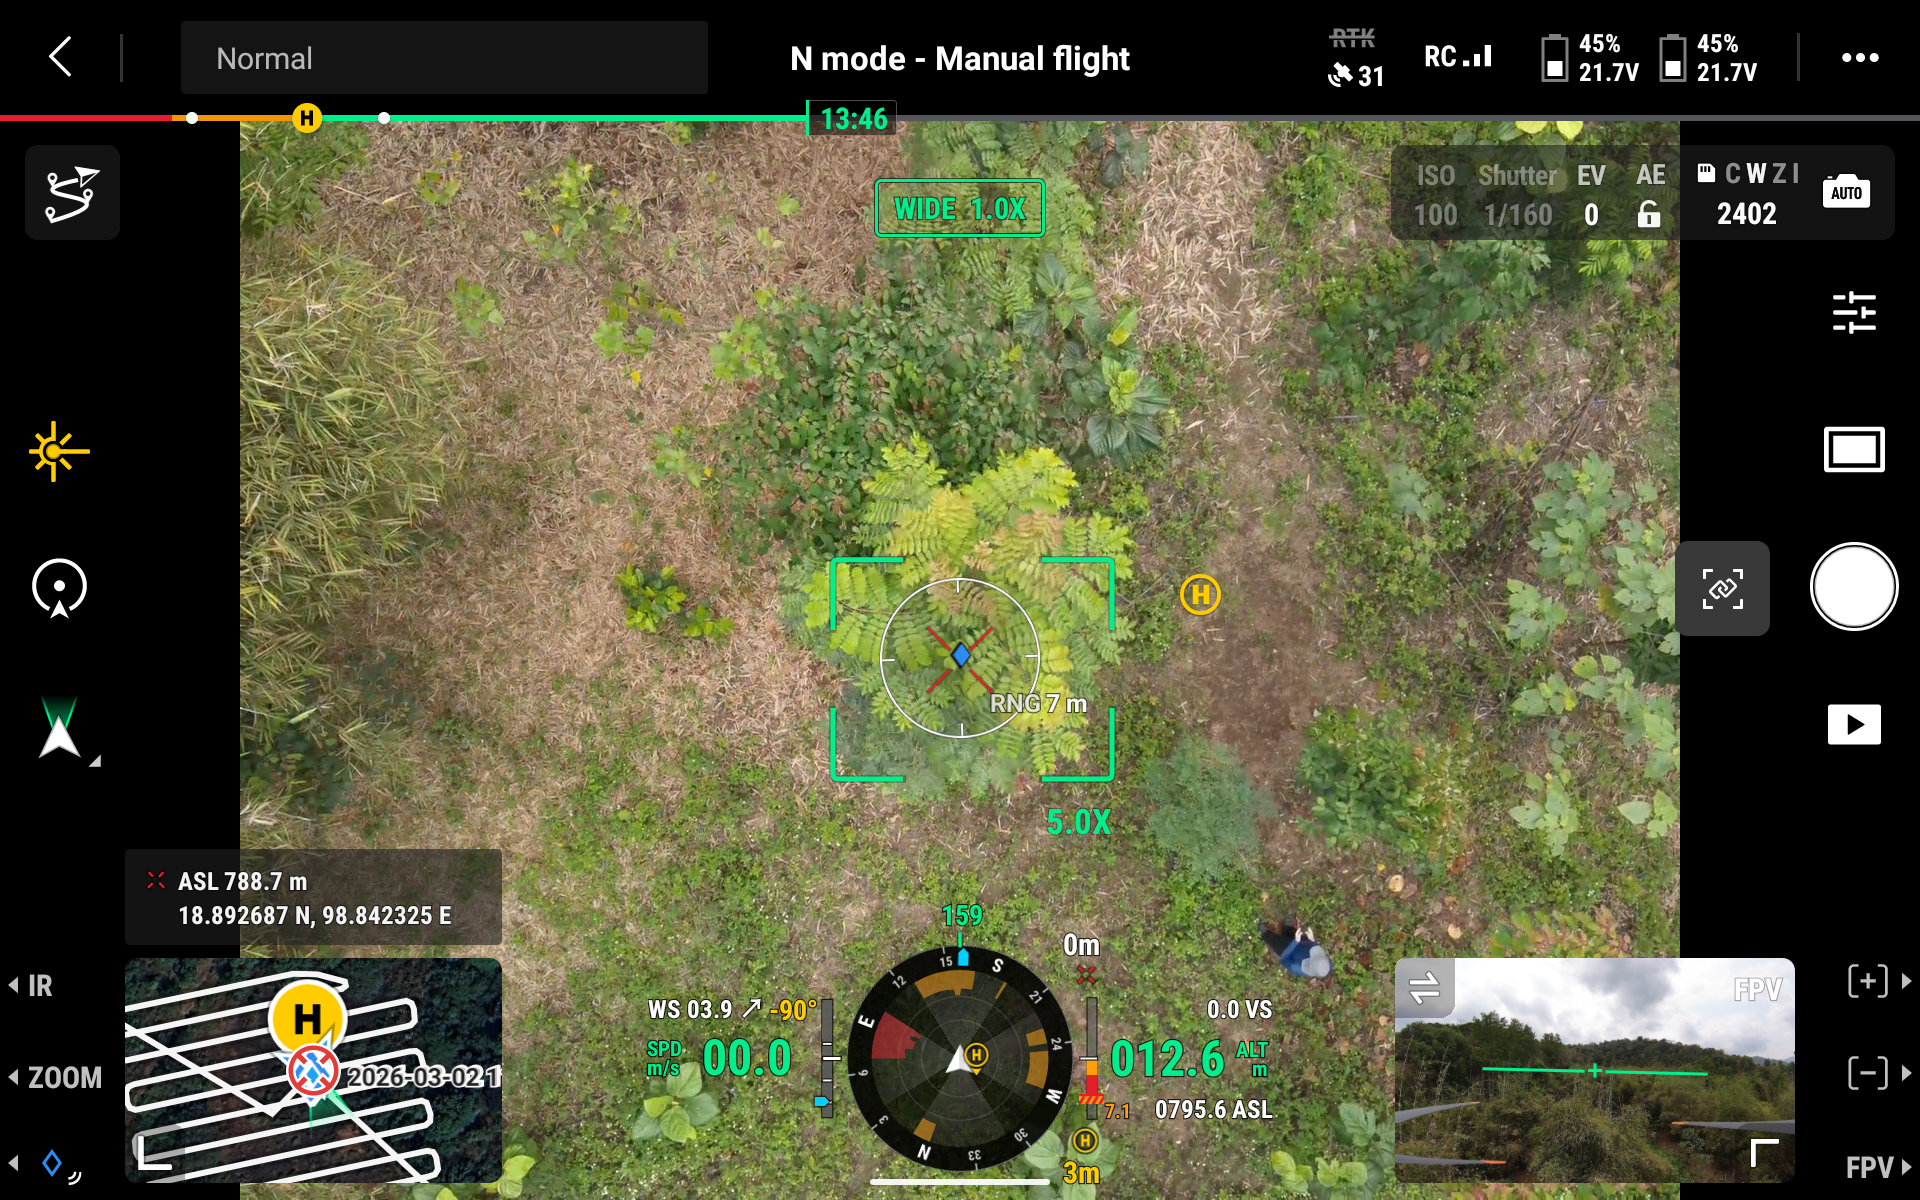
\includegraphics[width=0.6\linewidth]{fig/vps_tree1.png}
    \caption{ภาพหน้าจอรีโมทของโดรนขณะลอยตัวเหนือยอดไม้ของต้นที่ 1 เพื่อวัดระยะด้วยเซ็นเซอร์ VPS}
    \label{fig:vps_tree1}
\end{figure}

\begin{figure}[H]
    \centering
    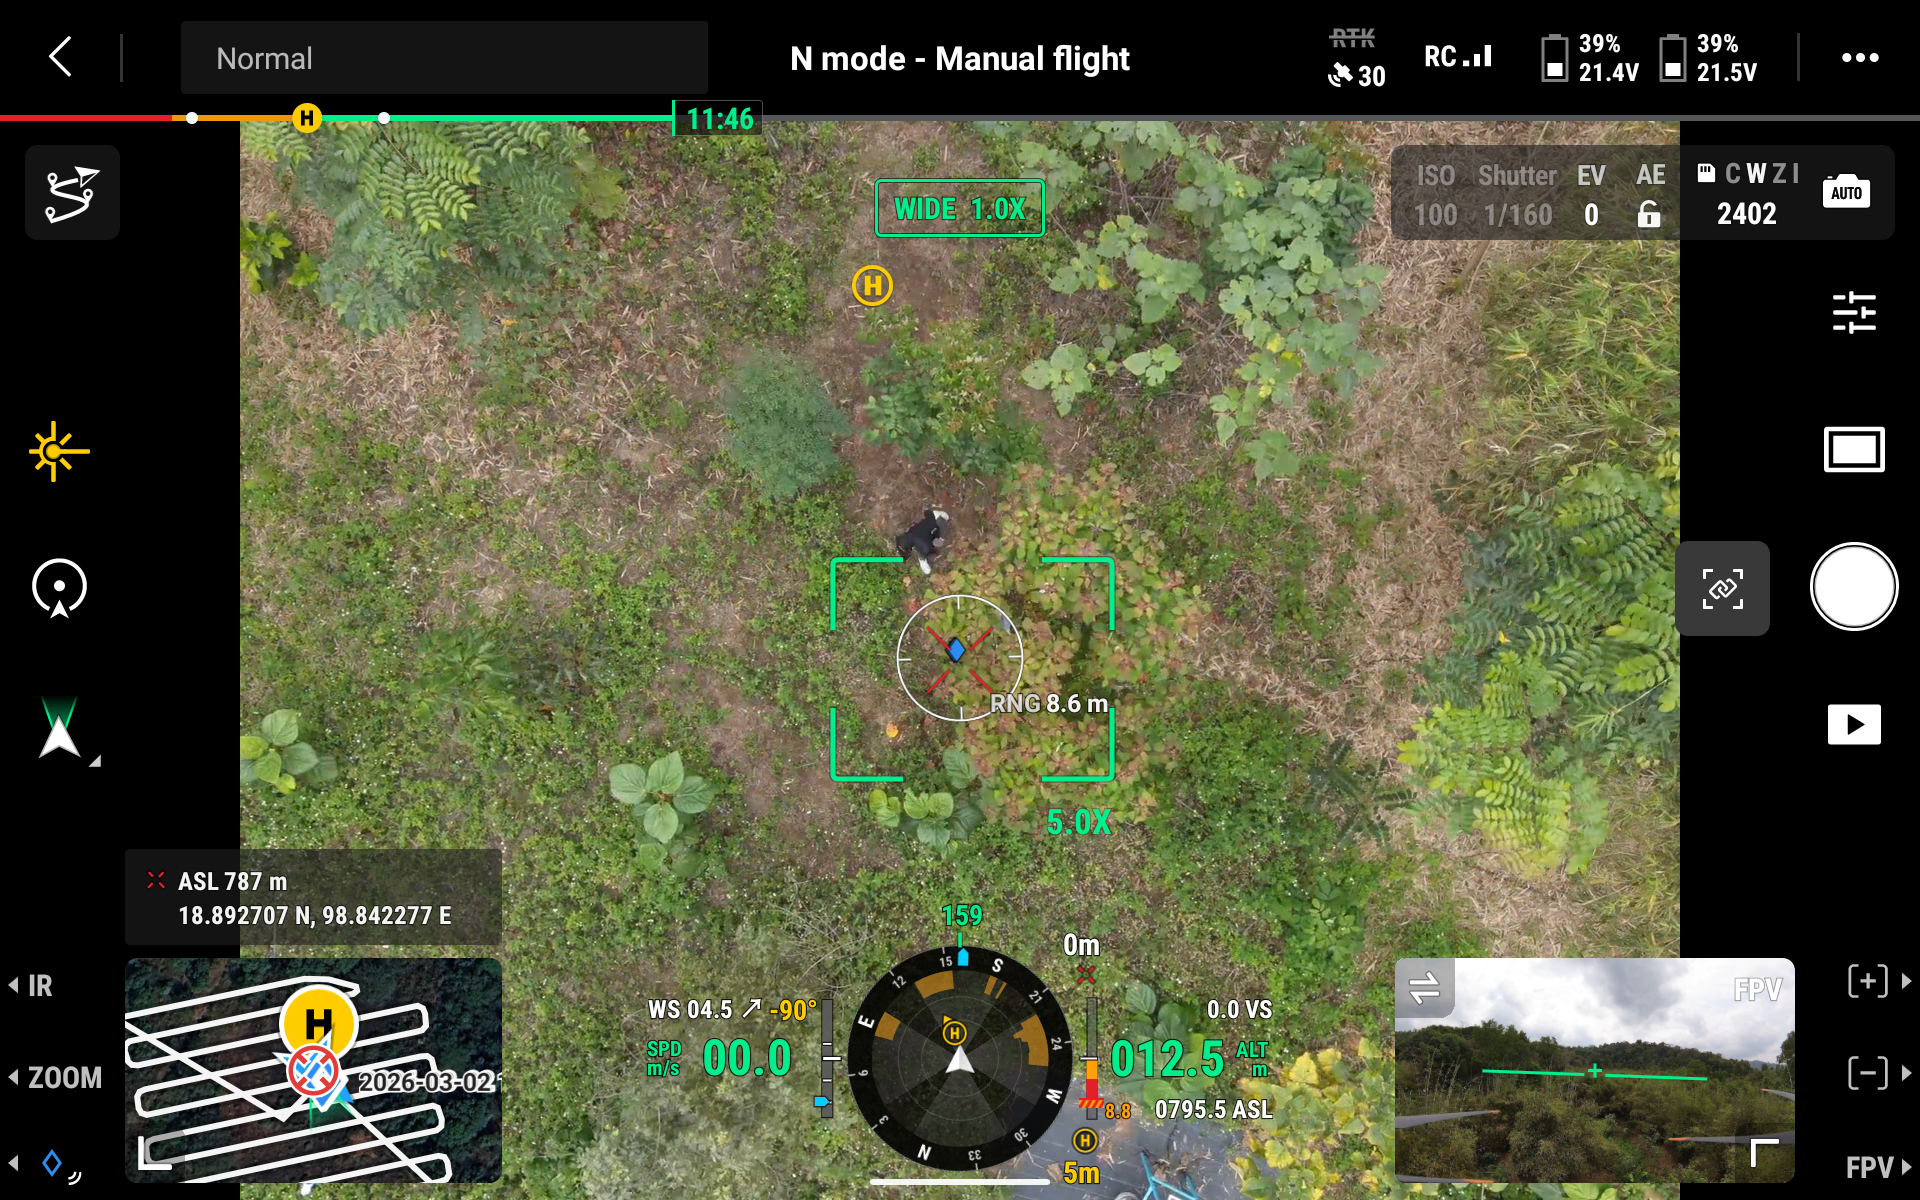
\includegraphics[width=0.6\linewidth]{fig/vps_tree2.png}
    \caption{ภาพหน้าจอรีโมทของโดรนขณะลอยตัวเหนือยอดไม้ของต้นที่ 2 เพื่อวัดระยะด้วยเซ็นเซอร์ VPS}
    \label{fig:vps_tree2}
\end{figure}

\begin{figure}[H]
    \centering
    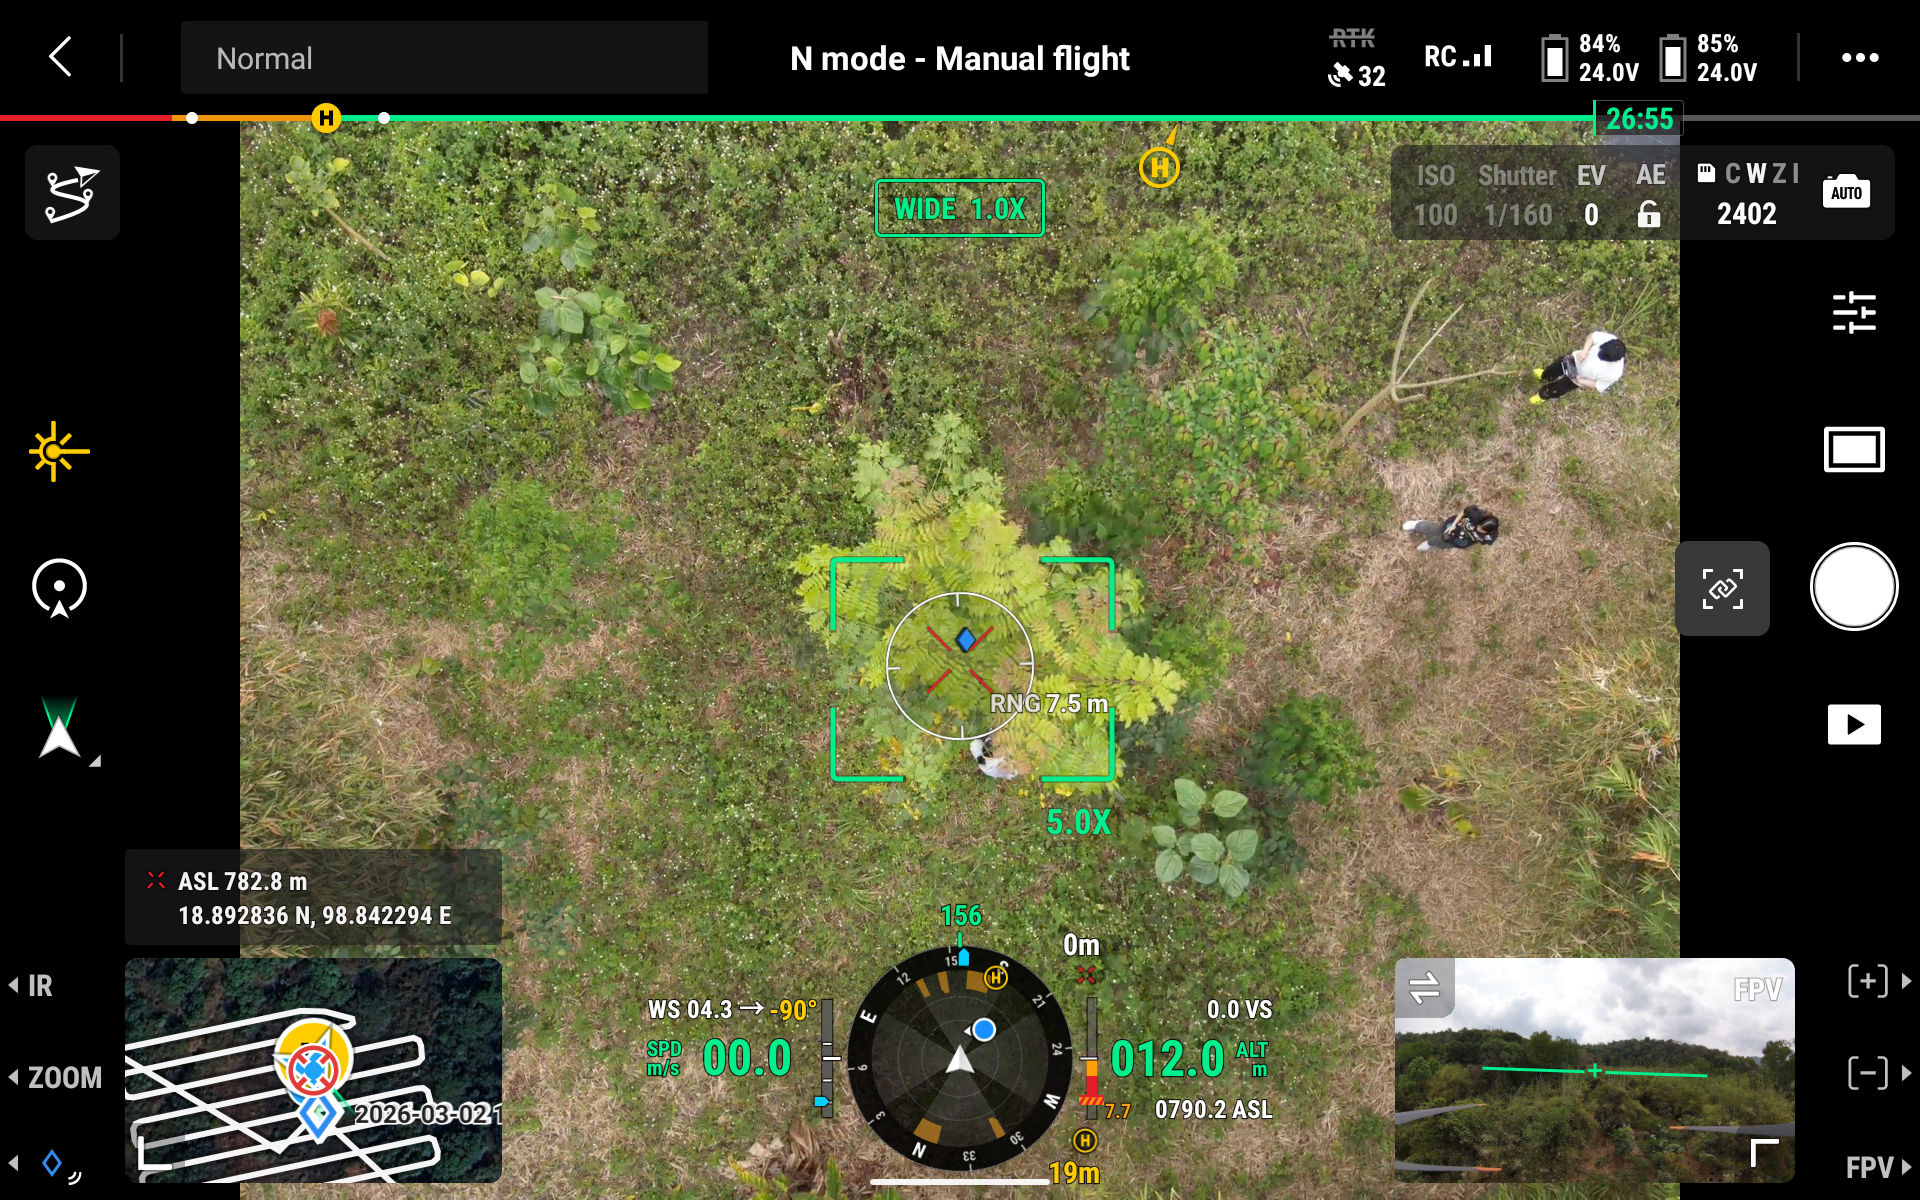
\includegraphics[width=0.6\linewidth]{fig/vps_tree3.png}
    \caption{ภาพหน้าจอรีโมทของโดรนขณะลอยตัวเหนือยอดไม้ของต้นที่ 3 เพื่อวัดระยะด้วยเซ็นเซอร์ VPS}
    \label{fig:vps_tree3}
\end{figure}

\section{ภาพการวัดความสูงจาก WebODM}
\begin{figure}[H]
    \centering
    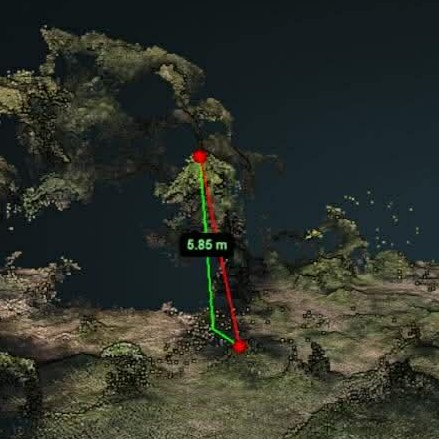
\includegraphics[width=8cm]{fig/odm_tree1.jpg}
    \caption{ภาพจากซอฟต์แวร์ WebODM แสดงการใช้เครื่องมือวัดความสูงของต้นไม้ต้นที่ 1 จากข้อมูล 3D Point Cloud}
    \label{fig:odm_tree1}
\end{figure}

\begin{figure}[H]
    \centering
    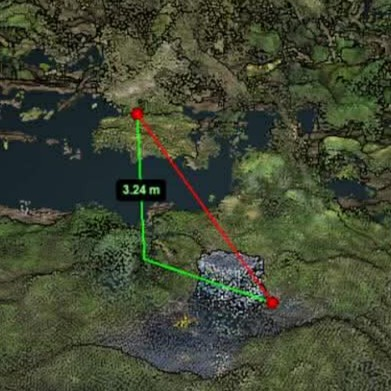
\includegraphics[width=8cm]{fig/odm_tree2.jpg}
    \caption{ภาพจากซอฟต์แวร์ WebODM แสดงการใช้เครื่องมือวัดความสูงของต้นไม้ต้นที่ 2 จากข้อมูล 3D Point Cloud}
    \label{fig:odm_tree2}
\end{figure}

\begin{figure}[H]
    \centering
    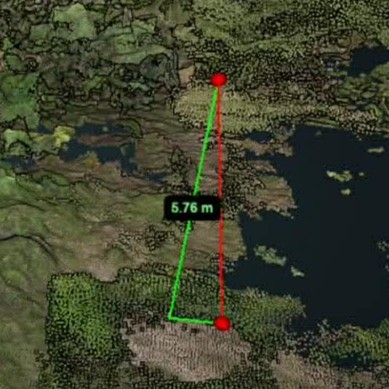
\includegraphics[width=8cm]{fig/odm_tree3.jpg}
    \caption{ภาพจากซอฟต์แวร์ WebODM แสดงการใช้เครื่องมือวัดความสูงของต้นไม้ต้นที่ 3 จากข้อมูล 3D Point Cloud}
    \label{fig:odm_tree3}
\end{figure}

\chapter{System Manual}
บทนี้นำเสนอคู่มือการใช้งานระบบสำหรับการวัดความสูงของต้นไม้ โดยอธิบายขั้นตอนการติดตั้งอุปกรณ์ การเตรียมระบบ และวิธีการใช้งานจริงในภาคสนาม เพื่อให้ผู้ใช้งานสามารถดำเนินการทดลองและเก็บข้อมูลได้อย่างถูกต้องและมีประสิทธิภาพ

\section{System Overview}
ระบบที่พัฒนาขึ้นมีวัตถุประสงค์เพื่อวัดความสูงของต้นไม้ โดยใช้การผสานเทคโนโลยี Ultra-Wideband (UWB) ร่วมกับอากาศยานไร้คนขับ (UAV) และการประมวลผลภาพถ่ายทางอากาศ ผู้ใช้งานสามารถวัดระยะทางระหว่างโดรนและจุดอ้างอิงบนพื้นดิน รวมถึงวัดระยะจากโดรนถึงยอดไม้ เพื่อนำไปคำนวณความสูงของต้นไม้ และเปรียบเทียบกับค่าความสูงจากแบบจำลองสามมิติ

\section{System Requirements}

\subsection{Hardware Requirements}
\begin{itemize}
    \item โมดูล ESP32 UWB จำนวน 2 ชุด (Tag และ Anchor)
    \item อากาศยานไร้คนขับ DJI M30T
    \item คอมพิวเตอร์สำหรับบันทึกและประมวลผลข้อมูล
    \item สายเชื่อมต่อสำหรับ ESP32
\end{itemize}

\subsection{Software Requirements}
\begin{itemize}
    \item Arduino IDE สำหรับอัปโหลดโปรแกรมลง ESP32
    \item Python สำหรับรันสคริปต์บันทึกข้อมูล
    \item WebODM สำหรับประมวลผลภาพถ่ายและสร้างแบบจำลองสามมิติ
\end{itemize}

\section{Hardware Setup}
การติดตั้งอุปกรณ์สามารถดำเนินการได้ดังนี้

\begin{enumerate}
    \item ติดตั้งโมดูล UWB Tag ไว้ใต้ตัวโดรนโดยใช้โครงยึด (Mount)
    \item วางโมดูล UWB Anchor บนพื้นดินบริเวณโคนต้นไม้เป้าหมาย
    \item เชื่อมต่อ Anchor กับคอมพิวเตอร์ผ่านพอร์ต USB
\end{enumerate}

\section{Software Setup}
การเตรียมระบบซอฟต์แวร์ประกอบด้วยขั้นตอนดังนี้

\begin{enumerate}
    \item อัปโหลดโปรแกรม \texttt{anchor.ino} ลงในอุปกรณ์ Anchor
    \item อัปโหลดโปรแกรม \texttt{tag.ino} ลงในอุปกรณ์ Tag
    \item ตรวจสอบหมายเลขพอร์ต (COM Port) ของอุปกรณ์ ESP32
    \item แก้ไขค่า \texttt{PORT} ในไฟล์ \texttt{write\_file.py} ให้ตรงกับพอร์ตที่ใช้งาน
    \item รันสคริปต์ \texttt{write\_file.py} เพื่อเริ่มบันทึกข้อมูล
\end{enumerate}

\section{System Operation}
ขั้นตอนการใช้งานระบบในภาคสนามมีดังนี้

\begin{enumerate}
    \item เปิดระบบ UWB และตรวจสอบการเชื่อมต่อระหว่าง Tag และ Anchor
    \item บินโดรนขึ้นไปลอยตัวเหนือยอดไม้เป้าหมาย
    \item อ่านค่าระยะจากโดรนถึงยอดไม้จากหน้าจอรีโมท (VPS)
    \item รักษาระดับความสูงของโดรน และเคลื่อนที่ในแนวราบเพื่อวัดระยะด้วย UWB
    \item ตรวจสอบว่าระบบสามารถรับค่าระยะทางได้อย่างต่อเนื่อง
    \item บันทึกข้อมูลระยะทางลงในไฟล์ CSV
\end{enumerate}

\section{Data Collection Procedure}
การเก็บข้อมูลในการทดลองประกอบด้วยข้อมูลจากหลายแหล่ง ดังนี้

\begin{itemize}
    \item \textbf{ข้อมูลจาก UWB:} ระยะทางระหว่าง Tag และ Anchor ซึ่งถูกบันทึกในรูปแบบไฟล์ CSV
    \item \textbf{ข้อมูลจาก VPS:} ระยะจากโดรนถึงยอดไม้ ซึ่งอ่านค่าจากหน้าจอรีโมทของโดรน
    \item \textbf{ภาพถ่ายทางอากาศ:} ใช้สำหรับสร้างแบบจำลองสามมิติใน WebODM
\end{itemize}

ผู้ใช้งานควรทำการบันทึกค่าจาก VPS และเวลาที่สอดคล้องกับข้อมูลจาก UWB เพื่อใช้ในการวิเคราะห์ภายหลัง

\section{Data Processing}
หลังจากเก็บข้อมูลแล้ว สามารถดำเนินการประมวลผลได้ดังนี้

\begin{enumerate}
    \item นำข้อมูลระยะทางจากไฟล์ CSV มาวิเคราะห์
    \item คำนวณความสูงของต้นไม้โดยอ้างอิงจากสมการที่นำเสนอไว้ในบทที่ 3
    \item นำภาพถ่ายทางอากาศเข้าสู่ WebODM เพื่อสร้างแบบจำลอง 3D Point Cloud
    \item ใช้เครื่องมือวัดระยะใน WebODM เพื่อวัดความสูงของต้นไม้
    \item เปรียบเทียบค่าความสูงที่ได้จากทั้งสองวิธี
\end{enumerate}

\section{Troubleshooting}
ปัญหาที่อาจพบระหว่างการใช้งานระบบและแนวทางแก้ไขมีดังนี้

\begin{itemize}
    \item \textbf{ไม่สามารถวัดระยะ UWB ได้:} ตรวจสอบการเชื่อมต่อของ Tag และ Anchor และรีสตาร์ทอุปกรณ์
    \item \textbf{ค่าระยะทางไม่เสถียร:} อาจเกิดจากสัญญาณสะท้อน (Multipath) ควรปรับตำแหน่งอุปกรณ์หรือหลีกเลี่ยงสิ่งกีดขวาง
    \item \textbf{ข้อมูลไม่ถูกบันทึก:} ตรวจสอบพอร์ต Serial และการทำงานของสคริปต์ Python
\end{itemize}